\PassOptionsToPackage{svgnames}{xcolor}
\documentclass[12pt]{article}



\usepackage[margin=1in]{geometry}  
\usepackage{algorithm,algpseudocode}
\newcommand{\vars}{\texttt}
\newcommand{\func}{\textrm}
\usepackage{graphicx}             
\usepackage{amsmath}              
\usepackage{amsfonts}
\usepackage{framed}               
\usepackage{amssymb}
\usepackage{array}
\usepackage{amsthm}
\usepackage{multirow}
\usepackage[nottoc]{tocbibind}
\usepackage{bm}
\usepackage{enumitem}
\usepackage{tikz}
\usepackage{pdfpages}
\usepackage{tabularx}
\usepackage{verbatim}
\algdef{SE}[SUBALG]{Indent}{EndIndent}{}{\algorithmicend\ }%
\algtext*{Indent}
\algtext*{EndIndent}
\newcolumntype{C}[1]{>{\centering\let\newline\\\arraybackslash\hspace{0pt}}m{#1}}
\newcommand\norm[1]{\left\lVert#1\right\rVert}
\setlength{\parindent}{0cm}
\setlength{\parskip}{0em}
\newcommand{\ind}{\hspace*{15pt}}
\newcommand{\Lim}[1]{\raisebox{0.5ex}{\scalebox{0.8}{$\displaystyle \lim_{#1}\;$}}}
\newtheorem{definition}{Definition}[section]
\newtheorem{theorem}{Theorem}[section]
\newtheorem{notation}{Notation}[section]
\theoremstyle{definition}
\DeclareMathOperator{\arcsec}{arcsec}
\DeclareMathOperator{\arccot}{arccot}
\DeclareMathOperator{\arccsc}{arccsc}
\DeclareMathOperator{\spn}{Span}
\DeclareMathOperator{\diff}{d}
\DeclareMathOperator{\NP}{NP}
\DeclareMathOperator{\VP}{VP}
\DeclareMathOperator{\WhNP}{Wh-NP}
\DeclareMathOperator{\Aux}{Aux}
\DeclareMathOperator{\GerundVP}{GerundVP}
\DeclareMathOperator{\GerundV}{GerundV}
\DeclareMathOperator{\PP}{PP}
\DeclareMathOperator{\PreDet}{PreDet}
\DeclareMathOperator{\Det}{Det}
\DeclareMathOperator{\Noun}{Noun}
\DeclareMathOperator{\Nominal}{Nominal}
\DeclareMathOperator{\Verb}{Verb}
\newcommand{\x}{\mathbf{x}}
\newcommand{\y}{\mathbf{y}}
\setcounter{tocdepth}{1}
\begin{document}
\title{Revision notes - CS4248}
\author{Ma Hongqiang}
\date{November 18, 2019}
\maketitle
\tableofcontents

\clearpage
%\twocolumn
\section{Regular Expressions and Automata}
\begin{definition}[Regular Expression]
\hfill\\\normalfont Regular Expression is a formula for specifying a set of strings.
\end{definition}
\begin{definition}[RE Patterns]
\hfill\\\normalfont 
\begin{itemize}
	\item \texttt{*}: zero or more occurrences of the previous char or expression
	\item \texttt{+}: one or more occurrences of the previous char or expression
	\item \texttt{?}: exactly zero or one occurrence of the previous char or expression
	\item \texttt{\{n\}}: $n$ occurrences of the previous char or expression
	\item \texttt{\{n,m\}}: from $n$ to $m$ occurrences of previous char or expression
	\item \texttt{\{n,\}}: at least $n$ occurrences of the previous char or expression
	\item \texttt{.}: one occurence of any character
	\item \texttt{$\ast$}: an asterisk
	\item \texttt{\\.}: a period
	\item \texttt{\\?}: a question mark
	\item \texttt{\\n}: a newline
	\item \texttt{\\t}: a tab
	\item \texttt{[ArrayOfChars]}: any of the char in ArrayOfChars
	\item \texttt{[StartingChar-EndingChar]}: any of the char from StartingChar to EndingChar, inclusive
	\item \texttt{[\^ASetOfChar]}: not any of the character in the SetOfChar
	\item \texttt{\^}: Start of a line
	\item \texttt{\$}: End of a line
	\item \texttt{\\d}: Expands to \texttt{[0-9]}
	\item \texttt{\\D}: Expands to \texttt{[\^0-9]}, any non-digit
	\item \texttt{\\s}: white space
	\item \texttt{\\S}: non-whitespace
\end{itemize}
Operator Precedence Hierarchy (highest to lowest):
\begin{itemize}
	\item Parenthesis: \texttt{()}
	\item Counters: \texttt{* + ?\{ \}}
	\item Sequences/anchors
	\item Disjunction: \texttt{|}
\end{itemize}
\end{definition}
\begin{definition}[Finite State Automata]
\hfill\\\normalfont \textbf{function} \textsc{D-Recognize}(\textit{tape}, \textit{machine}) \textbf{returns} accept or reject\\
\ind \textit{index}$\leftarrow$Beginning of tape\\
\ind \textit{current-state}$\leftarrow$Initial state of machine\\
\ind \textbf{loop}\\
\ind \ind \textbf{if} End of input has been reached \textbf{then}\\
\ind \ind \ind \textbf{if} current-state is an accept state \textbf{then}\\
\ind \ind \ind \ind \textbf{return} accept\\
\ind \ind \ind \textbf{else}\\
\ind \ind \ind \ind \textbf{return} reject\\
\ind \ind \textbf{elsif} \textit{transition-table}[\textit{current-state},\textit{tape}[\textit{index}]] is empty \textbf{then}\\
\ind \ind \ind \textbf{return} reject\\
\ind \ind \textbf{else}\\
\ind \ind \ind \textit{current-state}$\leftarrow$ \textit{transition-table}[\textit{current-state},\textit{tape}[\textit{index}]]\\
\ind \ind \ind \textit{index}$\leftarrow$ \textit{index} + 1\\
\textbf{end}
\end{definition}
\begin{definition}[Finite State Automata]
\hfill\\\normalfont 
\begin{itemize}
	\item $Q$: a finite set of $N$ states $q_0,\ldots, q_{N-1}$
	\item $\Sigma$: a finite input alphabet of symbols
	\item $q_0$: the start state
	\item $F$: set of final states, $F\subseteq Q$
	\item $\delta(q,i)$: transition function between states. Given a state $q\in Q$ and input symbol $i\in \Sigma$, $\delta(q,i)$ returns a new state $q'\in Q$.
\end{itemize}
\end{definition}
\begin{definition}[Non-deterministic FSA]
\hfill\\\normalfont A non-deterministic FSA can have the following behavour:
\begin{itemize}
	\item At a state $q$, transit to more than one state given the same symbol.
	\item At a state $q$, transit to another state without consuming any symbol: $\epsilon$ transition.
\end{itemize}
NFSA accepts an input string if there is \textbf{at least some} path in the NFSA that leads to an accepting state \textbf{and} exhausting the input string.
\end{definition}
\clearpage
\section{Words}
\begin{definition}[Morpheme]
\hfill\\\normalfont Morpheme refers to the minimal meaning-bearing unit in a language.
\end{definition}
There are 2 classes of morphemes: stems and affixes. Affix can be prefix, suffix, infix and circumfix.\\
There are also 2 classes of behaviour in morphology:
\begin{itemize}
	\item Inflection
	\begin{itemize}
		\item Combine a stem and an affix to form a word in the same classes as stem.
	\end{itemize}
	\item Derivation
	\begin{itemize}
		\item Combine a stem and an affix to form a word in a different class
		\item Harder to predict the meaning of the derived form
	\end{itemize}
\end{itemize}
There are attempts in using algorithm to strip affixes from stems, like Porter Stemming Algorithm.
\begin{definition}[Tokenization]
\hfill\\\normalfont Text tokenization converts text to a more convenient, standard form. It could involve:
\begin{itemize}
	\item Clitic contractions: we're$\rightarrow$ we are.
	\item Choose a single normalized form for words with multiple forms.
	\item Case folding: convert all words to lower case.
	\item and more.
\end{itemize}
For Penn Treebank Tokenization Standard, it does the following
\begin{itemize}
	\item Seperate out clitics: doesn't -> does n't
	\item Keep hyphenated words together
	\item Separate out all punctuation symbols
\end{itemize}
\end{definition}
We may encounter spelling error in our text corpus, and we may do one of the following:
\begin{itemize}
	\item Non-word error detection
	\item Isolated-word error correction
	\item Context-sensitive error detection and correction
\end{itemize}
It is recognized that most misspelled words in human typewritten text are single-error misspellings:
\begin{itemize}
	\item Insertion
	\item Deletion
	\item Substitution
	\item Transposition
\end{itemize}
However, we also note that it is harder to detect cognitive error than typographic error, as cognitive error does not result in a non-word. \\
In the following, we assume that we will detect and correct non-word spelling errors, without using context. We will first propose candidates, and score them using
\[
\hat{c}=\arg\max_{c\in C}P(c\mid o)=\arg\max_{c\in C}P(o\mid c)P(c)
\]
where $c$ is a class(word), $C$ a set of classes and $o$ observation, i.e. the misspelled word. \\
It is of our interest to evaluate $P(o\mid c)$ and $P(c)$.\\
$P(c)$ can be calculated by 
\[
P(c)=\frac{C(c)}{N}
\]
if not smoothed, and
\[
P(c)=\frac{C(c)+\lambda}{N+B\lambda}
\]
if smoothed. Here $N=\sum_{i=1}^B C(c_i)$, where $B$ is the number of distinct $c$'s in $C$, and $\lambda$ is a small number. \\
For $P(o|c)$, an simplistic approach is to use 
\[
P(o\mid c)=\begin{cases}
\frac{\textit{sub}[m,l]}{C(l)}\;\;\text{ if substitution}\\
\frac{\textit{trans}[k,l]}{C(kl)}\;\;\text{ if transposition}\\
\frac{\textit{ins}[l,m]}{C(l)}\;\;\text{ if insertion}\\
\frac{\textit{del}[k,l]}{C(kl)}\;\;\text{ if deletion}
\end{cases}
\]
where
\begin{itemize}
	\item $\textit{sub}[m,l]$: number of times the correct letter $l$ is typed as $m$
	\item $\textit{trans}[k,l]$: number of times the correct letter sequence $kl$ is typed as $lk$
	\item $\textit{ins}[l,m]$: number of times the extraneous letter $m$ was inserted after $l$
	\item $\textit{del}[k,l]$: number of times the letter $l$ was deleted from the correct letter sequence $kl$.
\end{itemize}
\begin{theorem}[Minimum Edit Distance]
\hfill\\\normalfont Determine the number of edits(insertion/deletion).\\
Use dynamic programming to deal with this. Idea is 
\[
\texttt{distance}[i,j]=\min(\texttt{distance}[i-1,j] + 1, \texttt{distance}[i-1,j-1] + a[i]==b[j]? 0 : 2), \texttt{distance}[i,k-1]+1
\]
\end{theorem}
\clearpage
\section{N gram}
For $n$-gram language model, we want to use the previous $n-1$ words to predict the next word, so we are concerned about the probability
\[
P(w_n\mid w_1,\ldots, w_{n-1})
\]
and
\[
P(w_1,\ldots, w_n)
\]
\begin{definition}[Types, Tokens]
\hfill\\\normalfont Number of tokens $N$ refers to total number of running words.\\
Number of types $B$ refers to number of distinct words in a corpus. It is obvious that
\[
N=C(c_1) + \ldots + C(c_B)
\]
\end{definition}
\begin{theorem}[Evaluating {$n$}-gram probability]
\hfill \begin{align*}
&P(w_1, w_2,\ldots, w_N)\\
=&P(w_1)P(w_2\mid w_1)\cdots P(w_N\mid w_1,\ldots, w_{N-1})\\
=&\prod_{k=1}^NP(w_k\mid w_1,\ldots w_{k-1})
\end{align*}
\end{theorem}
\begin{theorem}[{$n$}-gram approximation]
\hfill \\\normalfont We can assume that $w_k$ only depends on its previous $n-1$ words, so
\[
P(w_k\mid w_1,\ldots, w_{k-1}) \approx P(w_k\mid w_{k-(n-1)},\ldots, w_{k-1})
\]
Especially, bi-gram(2-gram) approximation refers to
\[
P(w_1,\ldots, w_N) \approx \prod_{k=1}^N P(w_k\mid w_{k-1})
\]
For such $2$-gram estimation, we need to evaluate $P(w_k\mid w_{k-1})$ on the RHS. We can do
\[
P(w_k\mid w_{k-1}) = \frac{C(w_{k-1}w_k)}{C(w_{k-1})}
\]
More generally, we have
\[
P(w_k\mid w_{k-(n-1)},\ldots, w_{k-1}) = \frac{C(w_{k-(n-1)},\ldots, w_k)}{C(w_{k-(n-1)},\ldots, w_{k-1})}
\]
\end{theorem}
For training, we first choose a vocabulary. For any out-of-vocabulary word, we replace it with the unknown word $<UNK>$, and estimate the probability of $<UNK>$ like a regular word.
\begin{definition}[Perplexity]
\hfill\\\normalfont Let $m$ be a language model. Perplexity($PP$)is defined as
\[
PP=m(w_1,\ldots, w_n)^{-\frac{1}{n}}
\]
A better language model has a lower perplexity.
\end{definition}
\begin{theorem}[Add-1 Smoothed Bigram Probability]
\hfill\\\normalfont We can add-1 smooth the bigram probability
\[
P(w\mid w_0) = \frac{C(w_0w)+1}{C(w_0) + V}:=\frac{C^\ast(w_0w)}{C(w_0)}
\]
where $C^\ast(w_0w)=(C(w_0w)+1)\frac{C(w_0)}{C(w_0)+V}$.
We define discount $d$ as
\[
d:=\frac{C^\ast(w_0w)}{C(w_0w)}
\]
\end{theorem}
However, such smoothing is not ideal, since it will dilute the probability of existing bigrams by a lot, due to large value of $V$.
\begin{theorem}[Witten-Bell Smoothed Bigram Probability]
\hfill\\\normalfont Let $C(w_0)=\sum_{i=1}^T C(w_0w_i)$, where $T$ is the number of distinct word types \textit{following} $w_0$.\\
Define  $T+Z=V$, so $Z$ is the number of unseen bigram types following $w_0$.\\
We further assume $T(w_0)$ is the total \textit{count} of all unseen bigrams. Under this assumption,
\[
P(w\mid w_0)=\frac{C(w_0w)}{C(w_0)+ T(w_0)}\text{ if }C(w_0w)>0
\]
and
\[
P(w\mid w_0)=\frac{T(w_0)}{Z(w_0)(C(w_0)+T(w_0))}\text{ if }C(w_0w)=0
\]
\end{theorem}
\begin{theorem}[Estimating {$n$}-gram probability using interpolation]
\hfill\\\normalfont After we get $P(w_0)$ and $P(w_0\mid w_{-1})$ from training set, we can use development set to get
\[
\hat{P}(w_0\mid w_{-1})=\lambda_1 P(w_0\mid w_{-1}) + \lambda_2 P(w_0)
\]
where $\sum_{i}\lambda_i = 1$, and $\lambda_i$ is determined by maximising $\hat{P}$ in development set.\\
However, we may encounter the problem of not seeing $w_{-1}w_0$, so $P(w_0\mid w_{-1})$ is unknown. We can estimate it by using \textbf{backoff}:
\[
\hat{P}(w_0\mid w_{-1})=\begin{cases}
\tilde{P}(w_0\mid w_1)\text{ if }C(w_{-1}w_0)>0\\
\alpha(w_{-1})\cdot \tilde{P}(w_0)\text{ if }C(w_{-1}w_0)=0
\end{cases}
\]
where $\tilde{P}$ is the discounted probability.\\
As such, we can determine $\alpha(w_{-1})$ as
\[
\alpha(w_{-1})=\frac{1-\sum_{w_0: C(w_{-1}w_0)>0}\tilde{P}(w_0\mid w_{-1})}{1-\sum_{w_0: C(w_{-1}w_0)>0}\tilde{P}(w_0)}
\]
\end{theorem}
\begin{theorem}[Kneser-Ney Smoothing for Bigrams]
\[
P_{KN}(w_0\mid w_{-1})=\begin{cases}
\frac{C(w_{-1}w_0)-D}{C(w_{-1})}\text{ if }C(w_{-1}w_0)>0\\
\alpha(w_{-1})\frac{|\{w_{-1}': C(w_{-1}'w_0)>0\}|}{\sum_{w}|\{w_{-1}':C(w_{-1}'w)>0\}}\text{ if }C(w_{-1}w_0)=0
\end{cases}
\]
\end{theorem}
\begin{definition}[Entropy]
\hfill\\\normalfont Entropy measures uncertainty. Entropy $H$ of a random variable $X$ is
\[
H(X)=-\sum_{x\in X} p(x)\log_2p(x)
\]
\end{definition}
\begin{definition}[Entropy of a Sequence]
\hfill\\\normalfont Entropy of a random variable ranging over all finite sequences of words of length $n$ in a language $L$ is
\[
H(w_1,\ldots, w_n)=-\sum_{W_1^n\in L}p(W_1^n)\log_2p(W_1^n)
\]
And the entropy rate(per-word entropy) is $\frac{1}{n}H(W_1^n)$.
\end{definition}
\begin{definition}[Entropy of a Language]
\hfill\\\normalfont $H(L)=\lim_{n\to\infty} \frac{1}{n}H(w_1,\ldots, w_n)$.\\
By SMB theorem,
\[
H(L)=\lim_{n\to\infty}-\frac{1}{n}\log_2 p(w_1,\ldots, w_n)
\]
\end{definition}
\begin{definition}[Cross Entropy]
\hfill\\\normalfont Let $p$ be actual probability distribution, and $m$ a model of $p$. We have the cross-entropy of $m$ on $p$ to be $H(p,m) = \lim_{n\to\infty}-\frac{1}{n}\sum_{W\in L}p(w_1,\ldots, w_n)\log_2m(w_1,\ldots, w_n)$.\\
By SMB theorem, we have
\[
H(p,m)=\lim_{n\to\infty	}-\frac{1}{n}\log_2 m(w_1,\ldots,w_n)
\]
It is guaranteed that $H(p)\leq H(p,m)$, and difference is a measure of accuracy of the model.\\
We have, the perplexity of the model to be $2^H$.
\end{definition}
\clearpage
\section{Part-of-speech Tagging}
Part-of-speech(POS) gives information about a word and \textit{its neighbours}. Also, the same word in different POS may be pronouced differently.\\
POS can help decide the correct morphological affixes, provide useful information to other NLP components, and help to determine the structure of a sentence.\\
\begin{definition}[English POS]
\hfill\\\normalfont Classes of POS consists of open class and closed class.\\
Opem class consists of noun, verb, adjective and adverb.\\
Closed class include the rest, i.e. determiner, preposition, conjunction etc.
\end{definition}
\begin{definition}[Noun]
\hfill\\\normalfont Noun refers to people, places, things. It can occur with determiners, take possessives, and can occur in plural form.\\
There is proper nouns, which are capitalized names, and also common nouns.
\end{definition}
\begin{definition}[Verb]
\hfill\\\normalfont Verb refers to actions and processes. It can have the following morphological forms:
\begin{itemize}
	\item Non-3rd-person-singular
	\item 3rd-person-singular
	\item Present participle
	\item Past participle
\end{itemize}
There is a subclass of verbs called \textbf{auxilliaries} which is of closed class.
\end{definition}
\begin{definition}[Adjective, adverb]
\hfill\\\normalfont Adjective describe properties or qualities. Adverbs can be modifying something, directional, locative, temporal, degree or manner.
\end{definition}
\begin{definition}[Closed Class POS]
\hfill\\\normalfont
\begin{itemize}
	\item Prepositions: on, under, over.\\ Occur before noun phrases.
	\item Determiners: a, an, the. Often start a noun phrase.\\ Articles is a subtype of determiner, which can be either indefinite or definite.
	\item Pronouns: she, I, others. \\ An abbrevation for referring to some noun phrase or entit or event. There are personal pronouns, possessive pronouns and Wh-pronouns.
	\item Conjunctions: and, but, if. \\ Join 2 phrases, clauses or sentences. There are coordinating conjunctions like mentioned above, and subordinating conjunctions like that.
	\item Auxiliary verbs: can, may, should
	\item Particles: off, out, on. \\ Combine with a verb to behave as a semantic unit.
	\item Numerals: one, two first, second
\end{itemize}
There are also auxiliary verbs which are closed. They provide semantic features of the main verb. Examples are be, do, have, can etc.\\
Other closed classes include:
\begin{itemize}
	\item Existential there
	\item Interjections
	\item Negatives
	\item Politeness markers
	\item Greetings
\end{itemize}
\end{definition}
\begin{definition}[POS Tagging]
\hfill\\\normalfont POS tagging is a task which inputs a sentence $S$, and output one single best POS tag for each word in $S$.
\end{definition}
POS Tagging can be done using rule-based tagging, or stochastic HMM tagging.
\begin{theorem}[Rule Based Tagging]
\hfill\\\normalfont Rule based tagging happens in 2 stages.
\begin{enumerate}
	\item Use a dictionary to assign each word a list of potential POS.
	\item Use a large list of hand-written disambiguation rules to narrow down to a single best POS for each word.
\end{enumerate}
\end{theorem}
\begin{theorem}[Stochastic POS Tagging]
\hfill\\\normalfont Stochastic POS Tagging tries to obtain the best tagging by
\[
\hat{T} = \arg\max_T P(T\mid W) = \arg\max_T P(T,W)
\]
where $P(T,W)$ is defined as
\begin{align*}
P(T,W):&=P(\langle s\rangle, t_1, w_1,\ldots, t_T, w_T, \langle/s\rangle)\\
&=P(\langle s\rangle) P(t_1\mid \langle s\rangle ) P(w_1\mid \langle s\rangle, t_1) \ldots
\end{align*}
Here, we do the following approximation
\begin{itemize}
	\item $P(\langle s\rangle) = 1$.
	\item $P(t_1\mid \langle s\rangle, t_1, w_1, \ldots, t_{i-1}, w_{i-1}) \approx P(t_i\mid t_{i-1})$
	\item $P(w_i\mid \langle s\rangle, t_1, w_1, \ldots, t_{i-1}, w_{i-1}, t_i)\approx P(w_i\mid t_i)$.
	\item $P(\langle /s\rangle\mid \langle s\rangle, t_1, w_1, \ldots, t_T, w_T) \approx P(\langle /s\rangle\mid t_T)$.
\end{itemize}
As such, we have
\[
P(T,W)=(\prod_{i=1}^T P(t_i\mid t_{i-1})\cdot P(w_i\mid t_i))P(\langle /s\rangle\mid t_T)
\]
So we need to select $t_1, to t_T$ to maximise the above.
\end{theorem}
\begin{theorem}[Hidden Markov Models]
\hfill\\\normalfont Given the assumptions above, we can use Hidden Markov Model to compute the probability above by treating tags as states, and words as observations\\
We define $Q = q_1\ldots q_N$ to be a set of $N$ states. 
Let $A = (a_{ij})_{1\leq i,j\leq n}$ be a transition probability matrix. 
Let $O=o_1\ldots o_T$ to be a sequence of $T$ observations, each one drawn from a vocabulary $V=v_1,\ldots,v_V$.\\
Let $B=b_i(o_t)$ to be a sequence of \textbf{obseration likelihood}, each expressing the probability of an observation $o_t$ being generated from a state $i$.\\
Let $q_0$ and $q_F$ to be a special start, and end state, together with $a_{01}\ldots a_{0n}$ out of start state, and $a_{1F}\ldots a_{nF}$ into the end state.\\
We clearly have
\[
\sum_{j=1}^n a_{ij}=1
\]
and
\[
\sum_{o_t\in V}b_i(o_t)=1
\]
Here, we want to determine the most probable state sequence. We can do so in $O(T\cdot N^2)$ using Viterbi algorithm. Viterbi algorithm relies on the fact:
\[
v_t(j) = \max_{1\leq i\leq N} v_{t-1}(i)a_{ij}b_j(o_t)
\]
\begin{figure}[h]
\centering
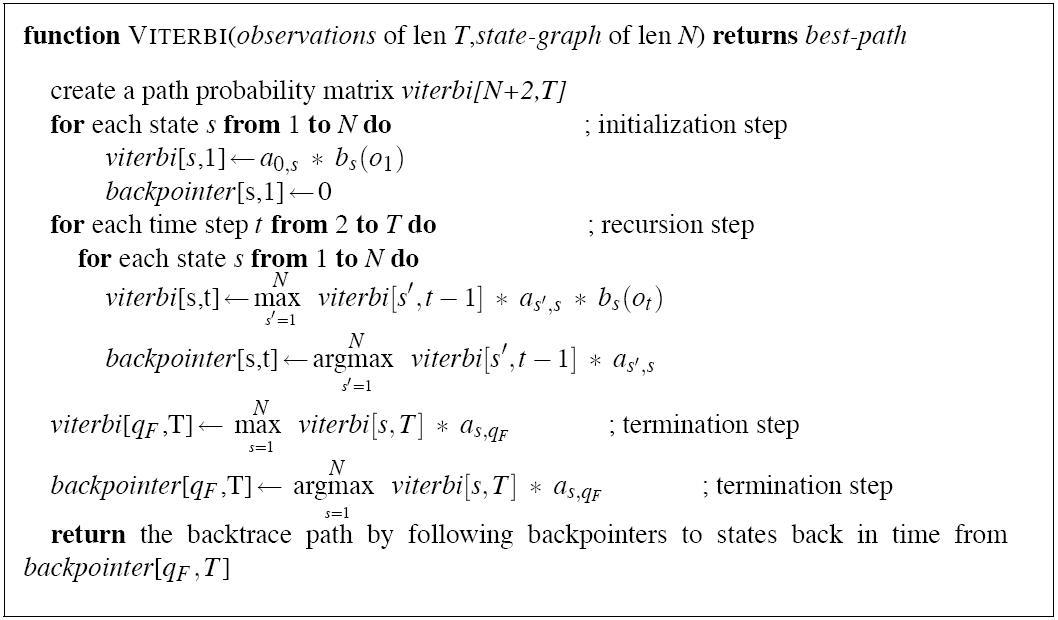
\includegraphics[width=\textwidth]{pos_tagging.jpg}
\end{figure}
\end{theorem}
\clearpage
\section{Linear Models}
\begin{definition}[Linear Model]
\hfill\\\normalfont A linear model refers to $f(\x) = \x\cdot \mathbf{W} + \mathbf{b}$, where $\x$ is the input, and $W\in\mathbb{R}^{d_{in}\times d_{out}}, b\in\mathbb{R}^{d_{out}}$ are parameter of the linear model.
\end{definition}
\begin{definition}[Binary Classification]
\hfill\\\normalfont If $b\in\mathbb{R}^1$, by letting $\hat{y}:=\text{sign}(f(\x))$, we can use such a linear model for a binary classification. Note, $\text{sign}(x)$ returns $1$ if $x\geq 0$ and $-1$ otherwise.
\end{definition} 
\begin{definition}[Log-linear Binary Classification]
\hfill\\\normalfont Instead of such an absolute binary classification using sign function, we can use sigmoid function $\sigma(x)=\frac{1}{1+e^{-x}}$, and
\[
P(\hat{y}=1\mid \x)=\sigma(f(\x))\;\;\;\;P(\hat{y}=0\mid \x)= 1-\sigma(f(\x))
\]
\end{definition}
\begin{definition}[Multi-class Classification]
\hfill\\\normalfont We can classify an $\x$ to one of the many possible($>2$) classes. \\
To do so, we can use a linear classifier, by letting $\hat{\y}:=f(\x)=\x\mathbf{W}+\mathbf{b}$, where $\y$ represents the probability of different classes. \\
Therefore, the prediction is $\arg\max_i \hat{\y}_i$.\\

We can also use \textbf{softmax} function defined as
\[
\text{softmax}(\x)_i = \frac{e^{\x_i}}{\sum_{j}e^{\x_i}}
\]
as a generator of a probability from $\hat{y}$.\\
Let $\hat{\y}=\text{softmax}(\x\mathbf{W}+\mathbf{b})$. Then $\hat{\y}_i$ is the probability of class $i$.
\end{definition}
\begin{definition}[Training as Optimization]
\hfill\\\normalfont We hope to find a function $f$, such that predictions $\hat{\y}:=f(\x)$ is accurate over the training set. To do so, we need to have a loss function $L(\hat{\y},\y)$ to quantify the loss suffered due to inaccurate prediction $\hat{\y}$.\\
As such we need to find parameters $\Theta$ that minimize the sum of loss fucntion and regularization term:
\[
\hat{\Theta}:=\arg\min_{\Theta}(\frac{1}{n}\sum_{i=1}^n L(f(\x_i;\Theta), \y_i)+\lambda R(\Theta))
\]
Regularization is to control the complexity of the parameter values and avoid overfitting. $\lambda$ can be used to control the extent of regularization and can be set manually based on development set.
\end{definition}
Following are some common loss functions
\begin{definition}[Binary Cross-entropy loss]
\hfill\\\normalfont Binary Cross-entropy loss is used in binary classification with conditional probability output, where $y\in{0,1}$ and $\hat{y}\in(0,1)$:
\[
L_{\text{logistic}}(\hat{y},y)=-y\log \hat{y}-(1-y)\log(1-\hat{y})
\]
This loss function maximizes the log conditional probability $\log P(y\mid \x)$ for each training example $(\x, y)$.
\end{definition}
\begin{definition}[Categorical Cross-entropy Loss]
\hfill\\\normalfont Categorical cross-entropy loss is used on $\y:=(\y_1,\ldots, \y_n)$, a vector representing the true multinomial distribution over the labels $1$ to $n$, and $\hat{\y}:=(\hat{y}_1,\ldots, \hat{y}_n)$, the classifier's output transformed by \textbf{softmax}:
\[
L_{\text{cross-entropy}}(\hat{\y}, \y):=-\sum_{i}\y_i\log(\hat{\y}_i)
\]
For hard classification problem with a single correct class, then we only will have 1 terms on the RHS.
\end{definition}
\begin{definition}[Ranking Loss]
\hfill\\\normalfont In the event of only having positive training examples, and generating negative training examples by corrupting positive training examples, we need to aim for $f(\x)-f(\x')>1$, where $\x$ positive and $\x'$ corrupted. We can define the loss function as such to achieve this training goal:
\[
L_{\text{ranking}}(\x, \x')=\max\{0,1-(f(\x)-f(\x'))\}
\]
\end{definition}
And following are some regularisation technique.
\begin{definition}[Common Regularization Functions]
\begin{itemize}
	\item $L_2$ regularization: $R_{L_2}(\mathbf{W})=||W||_2^2:=\sum_{i,j}\mathbf{W}_{ij}^2$
	\item $L_1$ regularization: $R_{L_1}(\mathbf{W})=||W||_1 = \sum_{i,j}|\mathbf{W}_{ij}|$
	\item Elastic Net: $R_{\text{elastic-net}}(\mathbf{W})=\lambda_1R_{L_1}(\mathbf{W})+\lambda_2R_{L_2}(\mathbf{W})$
\end{itemize}
\end{definition}
\begin{definition}[Gradient Descent]
\begin{figure}[h]
\centering
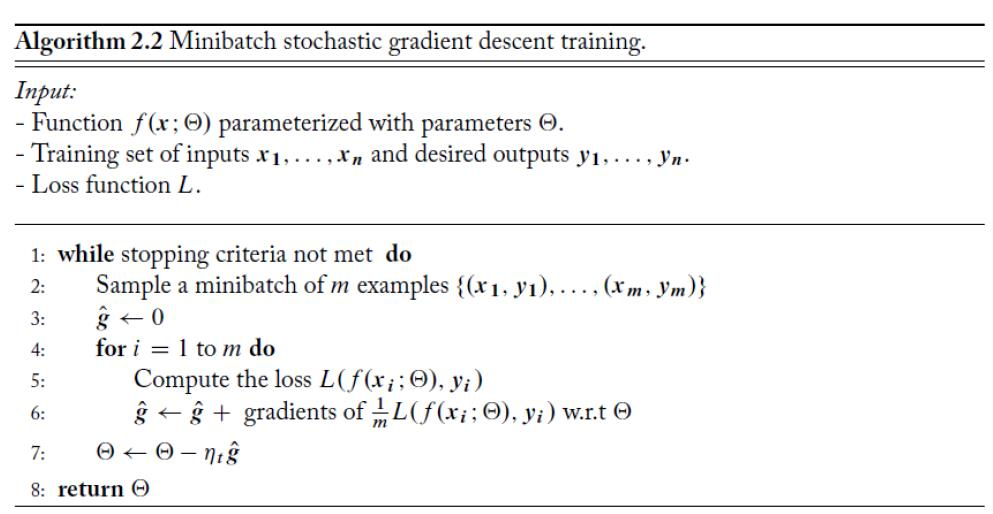
\includegraphics[width=0.9\textwidth]{gd.jpg}
\end{figure}
\end{definition}
\clearpage
\section{Feed-forward Neural Network}
Linear Model is not able to classify, without loss, a non-linear separable function. To resolve this work, we can apply to $\x$ a \textbf{non-linear input transformation} $\phi$, such that
\[
\hat{\y} = \phi(\x)\mathbf{W}+\mathbf{b}
\]
can be linearly separated. One of such function can be ReLU.
\begin{definition}[Multilayer perceptron]
\hfill\\\normalfont A multilayer perceptron with $k$ hidden layers is of the following form:
\[
NN_{k}(\x)=\mathbf{h}^{k}\mathbf{W}^{k+1}+\mathbf{b}^3 
\]
with 
\[
\mathbf{h}^i = g^i(\mathbf{h}^{i-1}\mathbf{W}^i + \mathbf{b}^i)
\]
and $h^0 = \x$.\\
We call $g^i$ activation function. Common activation functions can be sigmoid, $\tanh:=\frac{e^{2x}-1}{e^{2x}+1}$, hard $\tanh:=\begin{cases} -1 & x< -1 \\ 1 & x> 1 \\ x & \text{otherwise}\end{cases}$, ReLU$:=\max\{0,x\}$, etc.
\end{definition}
Similarly, as linear model, feed-forward neural network can also have binary classification, $k$-class classfication and softmax classfication.\\

A neural network can fit towards any function. To prevent a neural network from overfitting, we can randomly dropping half of the neurons in the neural network during stochastic gradient descent, i.e. after each layer of activation function.\\

For praciticalities, there are a few point to note:
\begin{itemize}
	\item Initialization: We can initialize a random weight matrix $\mathbf{W}\sim U(-\frac{\sqrt{6}}{\sqrt d_{in}+d_{out}}, +\frac{\sqrt{6}}{\sqrt d_{in}+d_{out}})$.
	\item We can have different random initializations and pick the best.
	\item We can combine multiple models in prediction, for example, through majority vote.
	\item For vanishing gradients, we can use specialized architecture such as LSTM.
	\item For exploding gradients, we can do $\hat{g}:=\min(\hat{g}, \frac{\text{threshold}}{||\hat{g}||}\hat{g})$.
	\item We need to experiment with learning rate.
\end{itemize}
\clearpage
\section{Neural Language Model}
Language Modelling is to assign a probability to a sequence of words, or assign a probability of a word following a sequence of words.\\
$N$-grams model requires intricate and manually designed smoothing schemes, and it is harder to scale to larger $n$-gram models, as number of observed $n$-gram grows at least multiplicatively when $n$ increases by 1. Also, $n$-gram has the problem with lack of generalization across contexts.
\begin{definition}[Neural Language Model]
\hfill\\\normalfont The input to multilayer perceptron is a sequence of $k$ words, and the output is a probability distribution over the next word.
\end{definition}
For example, the below is a neural language model with 2 hidden layer:
Let $\x=[v(w_1),\ldots, v(w_k)]$ be the sequence of $k$ words, where $v(\cdot)$ is the word embedding function. Let $\mathbf{h}=g(\x\mathbf{W}^1 + b^1)$, and $\hat{\y}=\text{softmax}(\mathbf{hW}^2 + \mathbf{b}^2)$.\\
For neural language model, since we need to have a word embedding of finite dimension, we need $V$ to be a finite vocabulary, including \texttt{UNK} for unknown words, \texttt{<s>} for sentence initial padding and \texttt{</s>} for end-of-sentence marking.\\

Training examples would be sequences of $k+1$ words from a corpus, where the first $k$ words are used as features, and last $(k+1)$th word as target label for classification. Due to such classification is categorical, we can use categorical cross-entropy loss $=\log(\hat{\y}_t)$, where $t$ is the index of the correct label.\\

Some drawbacks of neural network could be softmax, which is costly for very large vocabulary.\\

As you can see, we do need a word embedding function $v(\cdot)$ to kickstart our training. We can do one of the following to obtain an initial embedding:
\begin{itemize}
	\item random initialization
	\item supervised task-specific pretraining
	\item unsupervised pre-training
\end{itemize}
For \textbf{random initialization}, we can intiialize word vectors randomly. Suppose $d$ is the number of dimensions of a word vector after embedding, we can sample random numbers from $[-\frac{1}{2d}, \frac{1}{2d}]$ or other reasonable ranges.\\

For \textbf{supervised task-specific pre-training}, basically is to use the labelled training data in a large dataset in one task to pre-train word vector, and use that in training for a nother task.\\

For \textbf{unsupervised pre-training}, we use raw texts without human manual annotation. So we do need to predict a word based on its context, and also predict the context based on a word.
\begin{theorem}[Collobert and Weston]
\hfill\\\normalfont The context is surrounding words, i.e. $P(w_3\mid w_1w_2\cdot w_4w_5)$, and the Collobert Weston assign a score to a word, so we need to ensure that the correct word is assigned a score higher tthan incorrect words.
\[
s(w, c_{1:k})g(xU)\cdot v
\]
where $x=[v_c(c_1),\ldots, v_c(c_k); v_w(w)]$.\\
Here, $w$ is target word, $c_{1:k}$ a sequence of context words. $s$ is a score of a word-context pair.\\
$v_c(\cdot)$ is an embedding vector.\\
Loss function is a margin-based ranking loss function, with correct word-context pair above incoorect pairs with a margin of at least 1:
\[
L(w,c,w') = \max(0, 1-(s(w, c) - s(w', c)))
\] 
where $w'$ is a random chosen word.
\end{theorem}
\begin{theorem}[Word2Vec]
\hfill\\\normalfont Training for Word2Vec distinguishes a set $D$ of correct word-context pairs from a set $\bar{D}$ of incorrect word-context pairs.\\
The score is defined as $s(w,c)=\mathbf{w}\cdot\mathbf{c}$, where $\mathbf{w}, \mathbf{c}$ vectors of equal dimension.\\
The probability $P(D=1\mid w,c) = \frac{1}{1+e^{-s(w,c)}}$, and $P(D=0\mid w,c)=1-P(D=1|w,c)$.\\
The training objective is to maximize the log-likelihood of the data $D\cup \bar{D}$. So loss function is
\[
L=\sum_{(w,c)\in D}\log(P(D=1|w,c)) + \sum_{(w,c)\in \bar{D}}\log(P(D=0|w,c))
\]
The positive examples $(w,c)\in D$ is from a raw text corpus, whereas negative sampling is done by, for each $(w,c)\in D$, sample $k$ words and add each of these words $(w_i, c)$ as a negative example to $\bar{D}$.\\
Negative words are sampled, according to their corpus frequency: $\frac{\#(w)^{0.75}}{\sum_{w'}\#(w')^{0.75}}$. This gives higher relative weight to less frequent words.\\
For \textbf{CBOW}, suppose the context has $k$ words $c_{1:k}$, the context vector is computed by $\mathbf{c}:=\sum_{i=1}^k \mathbf{c}_i$, which means that the order of context words is ignored.\\
In other words, we have
\[
\log P(D=1| w, c_{1:k})=\log\frac{1}{1+e^{-\sum_{i=1}^k\mathbf{w}\cdot \mathbf{c_i}}}
\]
For \textbf{SkipGram}, We assume that each word in $c_{1:k}$ is independent of each other, so 
\[
P(D=1|w, c_{1:k})=\prod_{i=1}^k P(D=1|w, c_i) = \prod_{i=1}^k \frac{1}{1+e^{-\mathbf{w}\cdot \mathbf{c}_i}}
\]
After training, we will keep embeddings for the word, but not embeddings for the context.
\end{theorem}
\begin{theorem}[Word Similarity]
\hfill\\\normalfont Word Similarity can be measured via cosine similarity:
\[
\text{sim}_{\cos}(\mathbf{u}, \mathbf{v}) = \frac{\mathbf{u\cdot v}}{||u||_2||v||_2}
\]
\end{theorem}
Also, word analogy can be found via word vector algebra:
\[
\text{analogy}(mLw \to k: ?) = \arg\max_{v\in V\setminus\{m, w, k\}}\text{sim}_{\cos}(v, k-m+w)
\]
\clearpage
\section{CNN}
It is ideal if neural network can be specialised for dealing with language data, which is 
\begin{itemize}
	\item Sequential
	\item of Long distance dependency
\end{itemize}
CNN and RNN are useful.\\
CNN, convolutional neural networks identify information $n$-grams, and consider local ordering patterns. \\RNN, recurrent neural networks,
\begin{itemize}
\item Capture subtle patterns and regularities in sequences
\item Model non-Markovian dependencies
\item Consider infinite-window and zoom in on informative sequential patterns in the window.
\end{itemize}
 CNN and RNN are used as \textbf{feature extractors}, each producing a vector, or a sequence of vectors that is fed into further part of the network that eventually leads to prediction.\\
 The network is trained end-to-end, i.e. predicting part and CNN/RNN are trained together.
 \subsection{Convolutional Neural Networks}
 Naive solution to CBOW order-ignorance is to produce word vectors for bigrams, but it is problematic due to huge embedding matrix, and also different bigrams can be relevant, but are completely different bigrams.\\
 CNN serves as a feature-extracting architecture, that extract meaningful substructure useful for the overall prediction task.\\
 We focus on 1D convolutions:
 \begin{itemize}
 	\item We apply an \textbf{nonlinear, learned function} (filter) over each $k$-word sliding window in the sentence.
 	\item $l$ filters are applied to produce an $l$-dimentional vector for each sliding window of $k$ words.
 	\item A pooling operation combines the vector from different windows into a single $l$-dimensional vector.
 	\item This vector is fed into a neural network for prediction.
 \end{itemize}
 Filter functions learns to identify informative $k$-grams, whereas pooling enables focusing on the most important aspect of a sentence.\\
More formally, we have this formulation of CNN:
\begin{itemize}
	\item A sentence is a sequence of words $w_{1:n}$.
	\item Word embedding matrix $E$ is obtained for each word in $w_{1:n}$
	\item Sliding window size is $k$
	\item Define The window context $x_i = w_{i: i+ k - 1}$, where $w_j$ represents its \textbf{embedding}.
	\item Let $U=[u_1, \ldots, u_l]$ be $l$ different filters, each applicable on a vector of dimension $k$.
	\item We will have output from filters $p_i = g(x_i\cdot U + b)$, where $g$ is a non-linear activation function. \\
	$p_i$ is a collection of $l$ values representing the $i$th window, and each dimension of $p_i$ captures a different kind of indicative information.
	\item In total, we will have $m$ numbers of $p_i$ vectors.
	\begin{itemize}
		\item In narrow convolution, $m = n - (k - 1)$.
		\item In wide convolution, $m = n + (k-1)$, due to padding of $k-1$ words to each side.
	\end{itemize}
\end{itemize}
CNN also could accept multiple channels, say sequence of words, and also sequence of POS tags, and we can have different $p$'s for different channels, and we can combine the channels later arbitrarily, say by addition, or by vector.\\
As we can see, $p$ is sensitive to the identity and order of the words within a $k$ gram, but the same representation $p$ is extracted for the same $k$-gram regardless of its position within the sentence.\\
For pooling, we will combine $p_1,\ldots, p_m$ into a single vector $c$, where $c$ captures the essence of the important information in the sentence, and is fed downstream for prediction.\\
Training will turn downstream NN, $U$, $b$ and $E$ such that $c$ encodes information relevant to the prediction task.\\
\begin{definition}[Max Pooling]
\[
c_j = \max_{1\leq i \leq m }(p_i)_j
\]
\end{definition}
\begin{definition}[Average Pooling]
\[
c=\frac{1}{m}\sum_{i=1}^m p_i
\]
\end{definition}
CNN support hierarchical convolutions, where there is a hierarchy of convolutional layers:
\[
p_{1:m_1}^1 = \text{CONV}_{U^1, b^1}^{k_1}(w_{1:n})
\]
\[
\cdots
\]
\[
p_{1:m_r}^r = \text{CONV}_{U^r, b^r}^{k_r}(p^{r-1}_{1:m_{r-1}})
\]
Also, the sliding window can have custom \textbf{stride size} $s$, where window will be at $1, 1+s, 1+2s, \ldots$.\\
One observation is that if window size $k$ and stride size is $k-1$, there will be an exponential growth in the effective window size as a function of number of layers, from top to bottom.\\
Parameter tying is a technique where same $U, b$ are used in all the layers.\\
Skip connections is used in deep architectures, where $i$th layer is not only feed from $i-1$th layer but also from previous layers.
\clearpage
\section{RNN}
CNN has the problem of modelling of the word order is restricted to mostly local patterns.\\
RNN can overcome this problem.
\begin{figure}[h]
\centering
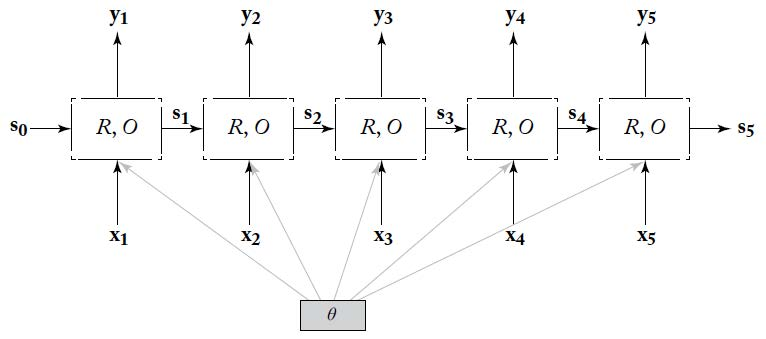
\includegraphics[width=0.7\textwidth]{rnn.jpg}
\end{figure}
We can represent RNN as
\begin{itemize}
	\item $RNN^{\ast}(x_{1:n}: s_0) = y_{1:n}$
	\item $s_i = R(s_{i-1}, x_i)$
	\item $y_i = O(s_i)$
\end{itemize}
The functions $R$ and $O$ are the same across the sequence positions.\\
The last $y_n$ encodes the entire input sequence and can be used for further prediction.\\
\begin{definition}[Simple RNN]
\hfill\\\normalfont 
\begin{itemize}
\item $s_i = R_{SRNN}(s_{i-1}, x_i):= g([s_{i-1}; x_i]W + b)$
\item $y_i = O_{SRNN}(s_i) = s_i$
\end{itemize}
\end{definition}
We can use RNN to predict an event $e$ given sequence $x_{1:n}$:
\[
P(e=j\mid x_{1:n}) = \text{softmax}(y_n\cdot W = b)_j
\]
RNN allows conditioning on the entire history withotu making Markov assumption.\\
RNN Training can be done via backpropagation through time, by adding a loss node after the last $y_i$.\\
RNN can be used as acceptor (in prediction), or as encoder, or as a transducer.\\
For RNN as transducer, we will produce an output $\hat{t}_i$ after each input $x_i$ is read. Therefore, we will have a local loss $L_{local}(\hat{t}_i, t_i)$, and the total loss
\[
L(\hat{t}_{1:n}, t_{1:n}) = \sum_{i=1}^n L_{local}(\hat{t}_i, t_i)
\]
One example, is to use RNN as a pos tagger, where each word input will have a tag output.
\begin{definition}[Bidirectional RNN]
\hfill\\\normalfont Bidirectional RNN uses both the previous and following words (context).
\begin{figure}[h]
\centering
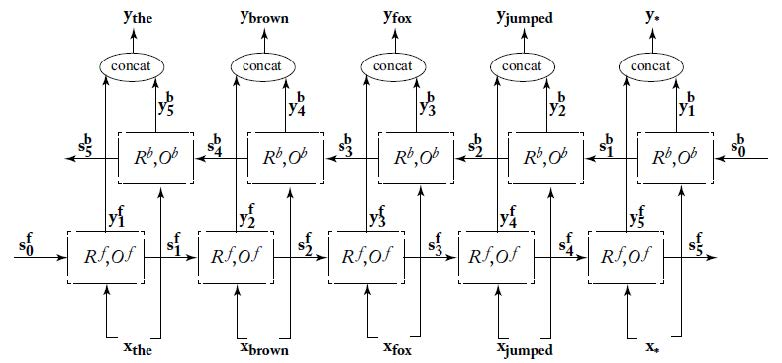
\includegraphics[width=0.7\textwidth]{birnn.jpg}
\end{figure}
\end{definition}
BiRNN is very effective for sequence tagging tasks.
\begin{definition}[Multilayered RNN]
\hfill\\\normalfont
We can stack multiple RNN together.
\begin{figure}[h]
\centering
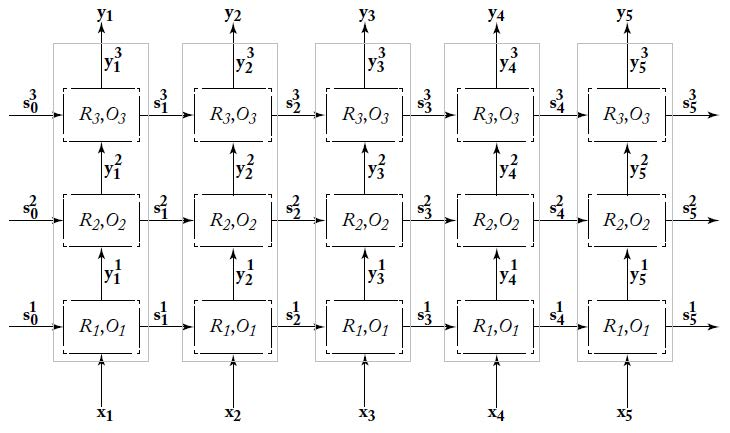
\includegraphics[width=0.7\textwidth]{multilayerrnn.jpg}
\end{figure}
\end{definition}
We can treat CBOW as RNN without taking into account order of words:
\begin{itemize}
	\item $s_i =R_{CBOW}(s_{i-1}, x_i) = s_{i-1} + x_i$
	\item $y_i = O_{CBOW}(s_i)=s_i$
\end{itemize}
Simple RNN is hard to train effectively, due to vanishing gradients. Gated architectures are designed to overcome this deficiency.
\begin{definition}[LSTM]
Long short-term memory is designed to solve vanishing problem.
\begin{itemize}
	\item $s_j = R_{LSTM}(s_{j-1}, x_j) = [c_j; h_j]$
	\item $i = \sigma(x_jW^{xi} + h_{j-1}W^{hi})$
	\item $f = \sigma(x_jW^{xf} + h_{j-1}W^{hf})$
	\item $o = \sigma(x_jW^{xo} + h_{j-1}W^{ho})$
	\item $z = \tanh(x_jW^{xz} + h_{j-1}^{hz})$
	\item $c_j = f\oplus c_{j-1} + i\oplus z$
	\item $h_j = p\oplus \tanh(c_j)$
	\item $y_j = O_{LSTM}(s_j) = h_j$
\end{itemize}
\end{definition}
RNN can be used for POS tagging:
\begin{itemize}
	\item $s$ to be the input sentence
	\item Let $w_i = c_1,\ldots, c_l$
	\item $c_i$ is the character embedding vector for $c_i$
	\item $x_i = \phi(s,i) = [E_{w_i}; RNN^f(c_{1:l}); RNN^b(c_{l:1})]$
	\item $p(t_i = j\mid w_1,\ldots, w_n) = \text{softmax}(MLP(biRNN(x_{1:n}, i)))_j$
	\item Trained with cross-entropy loss function
\end{itemize}
POS Tagging can include character embeddings, which take into account suffix, prefix, orthographic cues important for POS tagging.\\
POS tag prediction is conditioned on the entire input sentence.\\
RNN can be used as an acceptor, where it read an input sentence and produce a binary, or multiclass answer.\\
For example, given a sentence $s$, we can use RNN to classify $s$ as positive or negative.\\
\begin{itemize}
	\item $P(label = k \mid w_{1:n}) = \hat{y}_k, k = 1,2$
	\item $\hat{y} = \text{softmax}(MLP(RNN(x_{1:n})))$
	\item $x_{1:n} = (E_{w_1},\ldots,E_{w_n})$
\end{itemize}
But we can also use a bidirectional RNN.
\clearpage
\subsection{Formal Grammars of English}
\begin{definition}[Syntax]
\hfill\\\normalfont Syntax is relationship between words, including
\begin{itemize}
	\item Order of words
	\item Grouping of words
	\item Structure of sentences
\end{itemize}
\end{definition}
\begin{definition}[Constituent]
\hfill\\\normalfont A constituent is  a group of words that behaves as a single unit.
\end{definition}
A noun phrase is a sequence of words surrounding at least one noun.\\
\begin{definition}[Context-Free Grammar]
\hfill\\\normalfont 
It allows we to derive words from abstract data types. For example,
$NP\to Det Nominal \to Det Noun \to a Noun \to a flight$\\
The node $NP$ dominates all the nodes: $Det, Nominal, Noun, a, flight$.
The node $NP$ immediately dominates the nodes $Det, Nominal$.\\

The formal definition is $G=(N, \Sigma, P, S)$
\begin{itemize}
	\item $N$, a set of non-terminal symbols
	\item $\Sigma$, a set of terminal symbols
	\item $P$, a set of productions, each of the form $A\to \alpha$, where $A\in N$ and $\alpha \in (\sigma \cup N)^\ast$.
	\item A designated start symbol $S\in N$
\end{itemize}
If $A\to \beta$ is a production of $P$, and $\alpha$ and $\gamma$ are any strings in $(\Sigma\cup N)^\ast$, then $\alpha A\gamma$ directly derives $\alpha\beta\gamma$\\
Suppose that $\alpha_1,\ldots, \alpha_m$ are strings in $(\Sigma\cup N)^\ast$, $m\geq 1$, and
\[
\alpha_i\Rightarrow \alpha_{i+1}
\]
for $i= 1, \ldots, m-1$, then, $\alpha_1$ derives $\alpha_m$, or $\alpha_1\Rightarrow^\ast \alpha_m$.\\
The language generated by $G$, denoted by $L(G)$ is a set of strings composed of terminal symbols which can be derived from teh start symbol $S$ of $G$:
\[
L(G)=\{w\mid w\in \Sigma^\ast \text{ and } S\Rightarrow^\ast w\}
\]
Syntactic parsing is a mapping from a strin gof words to its parse tree.
\end{definition}
\begin{definition}[Strong Equivalence]
\hfill\\\normalfont Two grammars $G_1$ and $G_2$ are strongly equivalent if they generate the same set of strings $L(G_1) = L(G_2)$ and they assign the same phrase structure to each string, allowing only for renaming of non-terminal symbols.
\end{definition}
\begin{definition}[Weak equivalence]
\hfill\\\normalfont Two grammar are weakly equivalent if the generate the same set of strings but do not assign the same phrase structure to each string.
\end{definition}
\begin{definition}[Chomsky Normal Form]
\hfill\\\normalfont The grammar should be $\epsilon$-free, and each production of the grammar is either of the form $A\to BC$ or $A\to a$.
\end{definition}
Any CFG can be converted into a weakly equivalent CFG in Chomsky Normal Form.\\
\begin{definition}[Unit Production]
\hfill\\\normalfont A unit production is a production $A\to B$ where 
\begin{itemize}
	\item the RHS consists of a single non-terminal symbol $B$,
\end{itemize}
All other productions are non-unit productions.
\end{definition}
\begin{theorem}[Algorithm to convert CFG with no {$\epsilon$}production to CNF]
\hfill\\\normalfont
\begin{enumerate}
	\item Construct a new set of productions $P'$ by first including all non-unit productions
	\item For non-terminal symbols $A$ and $B$, if $A\to A_1\to \cdots \to B$, where $A_i$ are non-terminal symbols, then for each non-unit production $B\to\alpha$, add a new production $A\to \alpha$ to $P'$.
	\item Consider each production in $P'$ of the form $A\to X_1X_2\ldots X_m$, where $m\geq 2$. If $X_i$ is a terminal symbol $a$, introduce a new non-terminal symbol $C$ and a production $C\to a$. THey replace $X_i$ by $C$.
	\item For each production in $P'$ of the form $A B_1B_2B_3$, replace this production by $A\to B_1D_1$ and $D_1\to B_2B_3$
	\item Similar things should be done to $A\to $longer RHS sequences. $D_i$ will be new non-terminal symbols.
\end{enumerate}
\end{theorem}
There are four kinds of sentence-level constructions:
\begin{itemize}
	\item Declarative: $S\to \NP \VP$.
	\item Imperative: $S\to \VP$
	\item Yes-no-question: $S\to \Aux \NP \VP$
	\item Wh-question: $S\to \WhNP \VP$ or $S\to \WhNP \Aux \NP \VP$.
\end{itemize}
\begin{definition}[Clause]
\hfill\\\normalfont Clause form a complete thought, a node of a parser tree, below which the main verb of the clause has all of its arguments.
\end{definition}
\begin{definition}[Noun Phrase]
\hfill\\\normalfont Components of an NP:
\begin{itemize}
	\item Head: Central Noun
	\item Pre-nominal modifiers
	\item Post-nominal modifiers
	\item $Nominal \to Nominal Noun$
\end{itemize}
For Pre-head modifiers, it can be a determiner, a , the, or a possessive expression, like United's.\\
Determiners can be omitted, and there could be predeterminers coming before the determiners. $\NP\to \PreDet \NP$\\
Others can appear between the determiner and the head noun:
\begin{itemize}
	\item Cardinal numbers, 
	\item Ordinal numbers,
	\item Quantifiers,
	\item Adjective-phrase
\end{itemize}
So, we have
\[
NP\to (Det) (Card) (Ord) (Quant)(AP) Nominal
\]
For post-head modifiers, there could be
\begin{itemize}
	\item Prepositional phrases(PP): $\Nominal \to \Nominal \PP$ 
	\item Non-finite clauses $-ed, -ing$, or infinitive $\Nominal \to \Nominal \GerundVP$, where
	\begin{itemize}
		\item $\GerundVP \to \GerundV$
		\item $\GerundVP \to \GerundV \NP$
		\item $\GerundVP \to \GerundV \PP$
		\item $\GerundVP \to \GerundV \NP \PP$
		\item $\GerundV \to arriving |leaving | \ldots $
	\end{itemize}
	\item Relative clauses: $Nominal \to Nominal RelClause$, where
	\begin{itemize}
		\item $RelClause \to who VP$
		\item $RelClause \to that VP$
	\end{itemize}
\end{itemize}
\end{definition}
\begin{definition}[Agreement]
\hfill\\\normalfont Verbs can appear in 2 forms in the present tense:
\begin{itemize}
	\item For 3rd person, singular subjects
	\item For all other subjects
\end{itemize}
For yes-no questions, we have the following rules
\begin{itemize}
	\item $S\to 3sg\Aux 2sg\NP \VP$
	\item $S\to Non3sg\Aux Non3sg\NP \VP$
	\item $3sg\Aux \to does | has | can |\ldots$
	\item $Non3sg\Aux \to do | have | can |\ldots$
	\item $3sg\NP \to \Det Sg\Nominal$
	\item $Non3sg\NP \to \Det Pl\Nominal$
	\item $Sg\Nominal \to Sg\Noun$
	\item $Pl\Nominal \to Pl\Noun$
\end{itemize}
Note that determiner can also be singular(this) or plural(these).\\
Also, pronouns can be either nominative(I, he, she) or accusative(me, him, her).
\end{definition}
\begin{definition}[Verb Phrase]
\hfill\\\normalfont $VP\to \Verb | \Verb \NP | \Verb \PP | \Verb \NP \PP$.
A VP can have different kinds of constituents, depending on the verb.\\
Complements of a verb is constituents following a verb. A verb subcategorises for certain complements( what to expect). We define subcategorization frame, the possible sets of complements of a verb.\\
So depends on teh subcategorization frame, we can have this more fine grained notation:
\begin{itemize}
	\item $VP\to \Verb-with-no-comp$
	\item $VP \to \Verb-with-NP-comp \NP$
	\item $VP\to \Verb-with-S-comp\;S$
\end{itemize}
There are also auxiliary verbs:
\begin{itemize}
	\item Modal verbs: can, ...
	\item Perfect auxiliary: have
	\item Progressive auxiliary: be
	\item Passive auxiliary: be
\end{itemize}
An auxiliary verb places constraint on the form of the following verb, so it can be viewed as subcategorization:
\begin{itemize}
	\item Model-verb bare-stem
	\item Perfect-aux past-participle
	\item Progressive-aux presetn-participle
	\item Passive-aux past-participle
\end{itemize}
There are also orders between multiple auxiliary verbs: modal < perfect < progressive < passive.\\
A verb group is all auxiliary verbs plus the main verb.
\end{definition}
\begin{definition}[Coordination]
\hfill\\\normalfont NPs VPs and sentences can be joined with conjunctions(and, or).
\begin{itemize}
	\item $\NP\to \NP and \NP$
	\item $\VP \to \VP and \VP$
	\item $S\to S\;and\;S$.
\end{itemize}
\end{definition}
\begin{definition}[Treebank]
\hfill\\\normalfont Treebank is a corpus in which each sentence is syntactically annotated with a parse tree.
\end{definition}
Penn Treebank has traces (-NONE- nodes) to mark long-distance dependencies or syntactic movements.
It also have grammatical function tags, denoted as $-X$ after the main tag.
\begin{theorem}[Heads, Head Finding]
\hfill\\\normalfont Head is the word in the phrase that is grammatically most important. Heads are passed up a parse tree.\\
Each non-terminal in a parse tree is annotated with a word, which his its lexical head.\\
We need to manually identify one RHS constituent of a CFG rule as the head child of that rule. Lexical head of the parent is the lexical head of the head child.\\
We can have a head percolation table:
\begin{figure}[h]
\centering
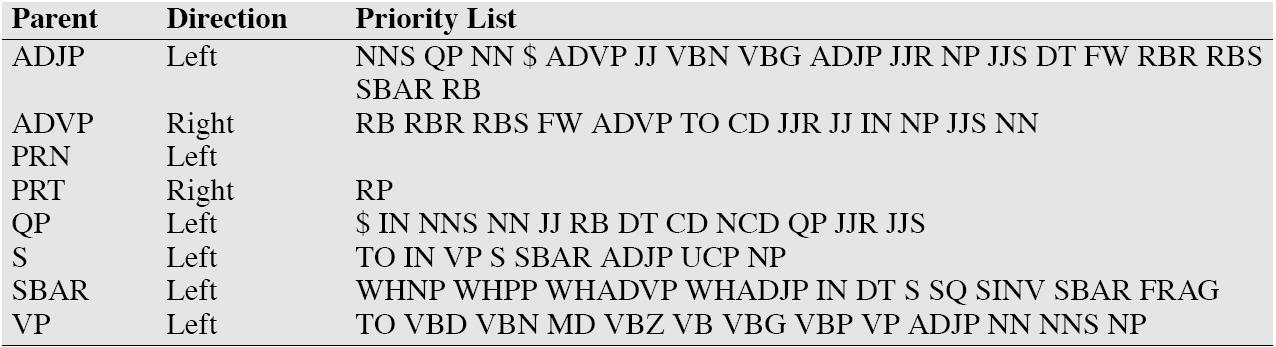
\includegraphics[width=0.7\textwidth]{headtable.jpg}
\end{figure}
For a CFG rule $VP\to Y_1\ldots Y_n$, start from left of $Y_1,\ldots Y_n$ to look for the first $Y_i$ of $TO$, and we try all the things on the priority list. If not found, return $Y_1$.
\end{theorem}
\begin{definition}[Dependency Grammars]
\hfill\\\normalfont Dependency grammars captures bianry relations between words in a sentence. It ignores constituent sand phrase structure rules.\\
It allows strong predictive power that a word has on its dependents. It also handlw eith ease languages with relatively free word order.
\end{definition}
We can transform a phrase structure parse into a untyped dependency parse using head percolation table.
\clearpage
\section{Syntactic Parsing}
We can parse using top-down parsing, by considering all possibilities starting $S$, and backtrack when failed.\\
We can also do bottom up parsing, and try combining them to get $S$.\\
There are pros and cons to both approach:
\begin{itemize}
	\item Top-down parsing
	\begin{itemize}
		\item Goal-directed search
		\item Never wastes time exploring trees that cannot result in an $S$
	\end{itemize}
	\item Bottom-up parsing
	\begin{itemize}
		\item Data-directed search
		\item Never suggests trees that are not grounded in the actual input sentence
	\end{itemize}
	\item Need to incorporate features of both
\end{itemize}
The problems of parsing is \textbf{structural ambiguity}:
\begin{itemize}
	\item Attachment ambiguity. \\
	There could be $VP(V, NP(NP, PP))$ or $VP(V, NP, PP)$, and $PP$ is used to describe different objects here.
	\item Noun-phrase bracketing ambiguity\\
	There could be $VP(V, NP(PNoun), NP(Nom))$ or $VP(V, NP(Nom(PNoun, Nom)))$, and the verb can have 2 noun phrases attached to it(do somebody something) or 1 noun phrases attached to it (do something).
	\item Coordination ambiguity\\
	Example: old men and women
\end{itemize}
Parsing can be considered as search, which involves searching the space of parse trees.\\
Agenda-based backtracking search leads to reduplication of work, as parsing of subtrees can be repeated.
\begin{definition}[Dynamic Programming Parsing Methods]
\hfill\\\normalfont 
\begin{itemize}
\item The CKY algorithm
\item Earley Algorithm
\item Chart parsing
\end{itemize}
\end{definition}
\begin{theorem}[CKY Algorithm]
\hfill\\\normalfont Bottom-up dynamic programming algorithm, which requires CFG to be in Chomsky Normal Form(CNF).\\
\textbf{function} \textsc{CKY-Parse}(words, grammar) \textbf{returns} table\\
\textbf{for} $j\leftarrow$ \textbf{from} 1 \textbf{to} Length(words) \textbf{do}\\
\ind table[$j-1$, $j$]$\leftarrow\{A\mid A\to \text{words}[j] \in \text{grammar}\}$\\
\ind \textbf{for} $i\leftarrow$ \textbf{from} $j-2$ \textbf{downto} $0$ \textbf{do}\\
\ind \ind \textbf{for} $k\leftarrow i + 1$ \textbf{ to } $j-1$ \textbf{do}\\
\ind\ind\ind table$[i,j]\leftarrow$table$[i,j]\cup\{A\mid A\to BC\in \text{grammar}, B\in \text{table}[i,k], C\in \text{table}[k,j]\}$\\

To return all possible parses,
\begin{itemize}
	\item Augment each entry such that each non-terminal is paired with pointers to the entries form which is was derived
	\item Permit multiple versions of the same non-terminal to be entered in an entry
\end{itemize}
\end{theorem}
\begin{theorem}[Earley Algorithm]
\hfill\\\normalfont Top-down dynamic programming algorithm. Uses a chart to store subtrees for each constituent.\\
Each possible subtree is only stored once only.\\
We have states, which is a CFG rule, with dots and indexes-pair. For example,
\[
S\to \cdot \VP [0,0]
\]
The presense of $S\to \alpha \cdot [0, N]$ in the list of states indicates a successful parse.\\
There are 3 operators:
\begin{itemize}
	\item Predictor
	\item Scanner
	\item Completer
\end{itemize}
Predictor creates new states representing top-down predictions/expectations. For example,
\begin{itemize}
	\item Given $S\to \cdot \VP [0,0]$,
	\item We add
	\begin{itemize}
		\item $\VP\to \cdot \Verb [0,0]$
		\item $\VP\to \cdot \Verb \NP[0,0]$
	\end{itemize}
\end{itemize}
Scanner uses the predicted POS to incorporate the next word. For example, 
\begin{itemize}
	\item Given state $\VP\to\cdot \Verb \NP [0,0]$
	\item Add new state: $\Verb \to \text{book} \cdot [0,1]$
\end{itemize}
Completer finds and advance all previously created states that were looking for this non-terminal at this position. For example
\begin{itemize}
	\item Givern state $\NP\to \Det \Nominal \cdot [1,3]$
	\item Find state $\VP\to \Verb \cdot \NP[0,1]$, and add the new state $\VP\to \Verb \NP\cdot [0,3]$.
\end{itemize}
\begin{figure}[h]
\centering
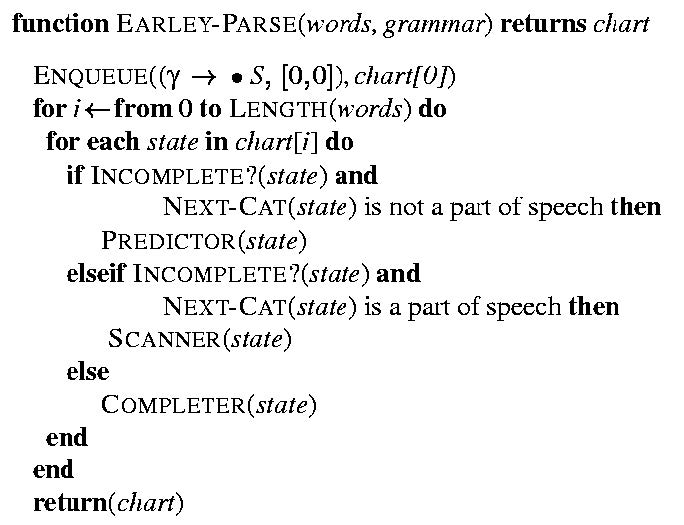
\includegraphics[width=0.6\textwidth]{earley.jpg}
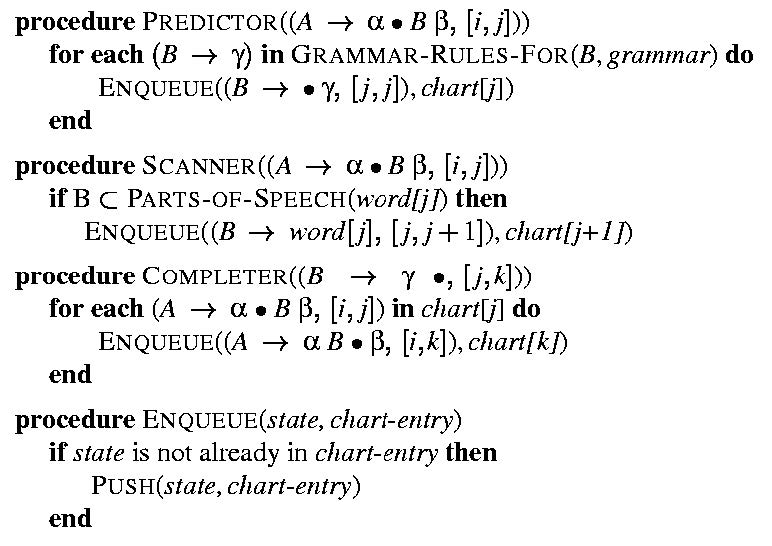
\includegraphics[width=0.6\textwidth]{earley2.jpg}
\end{figure}
\end{theorem}
\begin{theorem}[Chart Parsing]
\hfill\\\normalfont Chart parsing allows a flexible and dynamic order of processing the chart entries through an explicit agenda.\\

\textbf{function} Chart-Parse(words, grammar, agenda-strategy) \textbf{returns} chart\\
Initialize(chart, agenda, words)\\ 
\textbf{while} agenda\\
\ind current-edge $\leftarrow$ Pop(agenda)\\
\ind Process-Edge(current-edge)\\
return (chart)\\


\textbf{procedure} Process-Edge(edge)\\
\ind Add-to-Chart(edge)\\
\textbf{if} Incomplete?(edge)\\
\ind Forward-Fundamental-Rule(edge)\\
\textbf{else}\\
\ind Backward-Fundamental-Rule(edge)\\
Make-Predictions(edge)\\

\textbf{procedure} Forward-Fundamental-Rule($A\to \alpha B\beta,[i,j]$)\\
\textbf{for each} ($B\to \gamma\cdot, [j,k])$ \textbf{in} chart\\
\ind Add-to-Agenda($A\to\alpha B\cdot \beta,[i,k])$\\

\textbf{procedure} Backward-Fundamental-Rule($B\to \gamma\cdot, [j,k]$)\\
\textbf{for each} ($A\to\alpha B\beta, [i,j])$ \textbf{in} chart\\
\ind \textbf{Add-to-Agenda}($A\to\alpha B\cdot \beta, [i,k]$)\\

\textbf{procedure} Add-to-Chart(edge)\\
\textbf{if} edge is not already in chart \textbf{then}\\
\ind add edge to chart\\

\textbf{procedure} Add-to-Agenda(edge)\\
\textbf{if} edge is not already in agenda \textbf{then}\\
\ind apply(agenda-strategy, edge, agenda)\\

\textbf{procedure} Make-Prediction(edge)\\
\textbf{if} Top-Down and Imcomplete?(edge)\\
\ind TD-Predict(edge)\\
\textbf{elseif} Bottom-up and Complete?(edge)\\
\ind BU-Predict(edge)\\

\textbf{procedure} TD-Predict($A\to \alpha\cdot B \beta, [i,j]$)\\
\textbf{for each}($B\to\gamma$) \textbf{in} grammar \textbf{do}\\
\ind Add-to-agenda($B\to\cdot \gamma, [j,j]$)\\

\textbf{procedure} BU-Predict($B\to \gamma\cdot, [i,j]$)\\
\textbf{for each}($A\to B\beta$) \textbf{in} grammar \textbf{do}\\
\ind Add-to-agenda($A\to\cdot B\cdot \beta, [i,j]$)\\
\end{theorem}
\clearpage
\section{Statistical Parsing}
Statistical parsing aims to resolve structural ambiguity, by choosing the most probable parse.
\begin{definition}[Probablistic Context-Free Grammar]
\hfill\\\normalfont Let $G=(N, \Sigma, P, S, D)$ be the PCFG, where
\begin{itemize}
	\item $N$ is a set of non-terminal symbols
	\item $\Sigma$ a set of terminal symbols, with $N\cap \Sigma = \varnothing$
	\item $P$, a set of productions, each of the form $A\to \alpha$, where $A\in N$ and $\alpha in (\Sigma \cup N)^\ast$
	\item $S\in N$, a designated start symbol
	\item $D$, a fucntion that assigns a probablity to each rule in $P$:
	\[
	P(A\to \alpha) \text{ or }P(A\to \alpha\mid A)
	\]
\end{itemize}
The score of a parse tree is provided by 
\[
P(T, S) = \prod_{n\in T}p(r(n))
\]
So 
\[
\hat{T}(S) = \arg\max_{T \text{ s.t. } S=\text{yield}(T)}P(T\mid S) = \arg\max P(T)
\]
\end{definition}
\begin{definition}[Probabilitistic CKY ALgorithm]
\hfill\\\normalfont PCKY requires PCFG to be in Chomsky Normal Form $A\to BC$ or $A\to \alpha$.\\
$\text{table}[i,j,A]$ stores the max probability for a constituent $A$ spanning word positions $i$ to $j$. So the probability of most probably parse is $\text{table}[0,n,S]$.\\


\textbf{function} PCKY(words, grammar) \textbf{returns} most probably parse and probability\\
\textbf{for} $j\leftarrow$ \textbf{from} 1 \textbf{to} length(word) \textbf{do}\\
\ind \textbf{for all} $\{A\mid A\to \text{words}[j] \in G\}$\\
\ind \ind $\text{table}[j-1,j,A]\leftarrow P(A\to \textbf{words}[j])$\\
\ind \textbf{for} $i\leftarrow$ \textbf{from} $j-2$ \textbf{downto} $0$ \textbf{do}:
\ind \ind \textbf{for} $k\leftarrow i + 1$ \textbf{to} $j-1$ \textbf{do}\\
\ind \ind \ind \textbf{for all} $\{A\mid A\to BC \in G\}$ \textbf{and} $\text{table}[i,k,B]>0$ \textbf{and} $\text{table}[k,j,C]>0$\\
\ind \ind \ind \ind \textbf{if} $\text{table}[i,j,A] < P(A\to BC)\times \text{table}[i,k,B]\times \text{table}[k, j, C]$ \textbf{then}\\
\ind \ind \ind \ind \ind $\text{table}[i,j,A]\leftarrow P(A\to BC)\times \text{table}[i,k,B]\times \text{table}[k, j, C]$\\
\ind \ind \ind \ind \ind $\text{back}[i,j,A]\leftarrow \{k, B, C\}$\\
\textbf{return} Build-Tree(back$[0, \text{length(words)}, S]$), table[0, length(words), $S$].
\end{definition}
To learn PCFG Rule Probabilities, we can estimate from parsed sentences(treebank):
\[
P(\alpha\to \beta\mid \alpha) = \frac{\#(\alpha\to\beta)}{\sum_{\gamma}\#(\alpha\to\gamma)} = \frac{\#(\alpha\to\beta)}{\#(\alpha)}
\]
THe problem of PCFG include
\begin{itemize}
	\item Poor independence assumptions\\
	The expansion of a non-terminal actually depends on its context. For example, $NP$ can be either pronoun or non-pronoun, and the expansion probability will differ. 
	\item Lack to sensitivity to words:
	\begin{itemize}
		\item Attachment ambiguity: Some words may attach to some other words in a fixed manner, and knowing such words will help in disambiguation.
		\item Coordination Ambiguity: It could have the same conditional probability due to the same set of grammar rules used, but many possibilities exist, in which only 1, in the correct structure, is correct.
	\end{itemize}
\end{itemize}
To resolve coordination ambiguity, we use \textbf{parent annotation}, i.e. for each tag, we include parent's tag also, if it is ambiguity.
\begin{figure}[h]
\centering
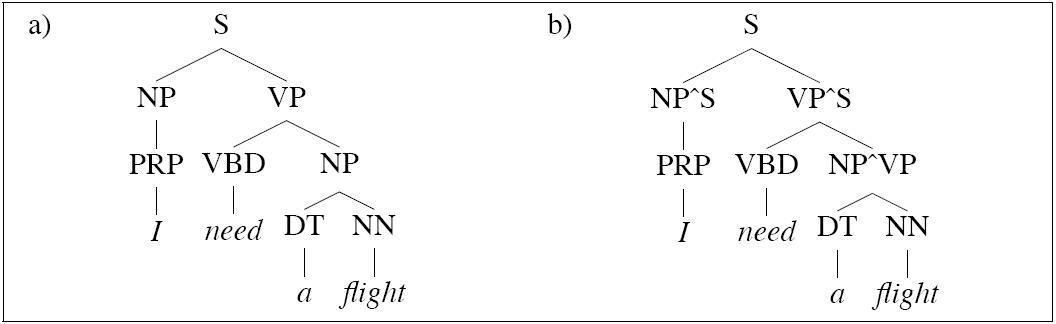
\includegraphics[width=0.7\textwidth]{parentanno.jpg}
\end{figure}
WE can also split non-terminals and preterminals:
\begin{itemize}
	\item Each non-terminal in a parse tree is annotated with a word(lexical head)
	\item Identify one RHS constituent of a  PCFG rule as the head child of that rule
	\item Lexcial head of the parent is the lexical head of the head child
\end{itemize}
This forms a probablistic lexicalized CFG, where we can capture dependencies between words.\\
The Collins Parser uses such probablistic lexicalized CFG.
\begin{definition}[Collins Parser Model 1]
\hfill\\\normalfont Each rule has the form $P(h)\to L_n(l_n)\cdots L_1(l_1)H(h)R_1(r_1)\ldots R_m(r_m)$, where $h, l_i, r_i$ is of the form $\langle \text{headword}, \text{headPOSTag}\rangle$.\\
$P(\text{RHS}\mid \text{LHS})$ is obtained by multiplying
\begin{itemize}
	\item $P_h(H\mid P, h)$: generate the head constituent
	\item $P_r(R_i(r_i)\mid H, P, h, \text{distance}_r(i-1))$: generate each right modifier
	\item $P_l(L_i(l_i)\mid H, P, h, \text{distance}_l(i-1))$: generate each left modifier
\end{itemize}
Herer, $P, L, H, R$ are the type.\\
$\text{distance}_\cdot (x)$ is a function of the surface string between head and the distance the tags crosses, and returns:
\begin{itemize}
	\item whether string is of length 0
	\item and whether string contain a verb
\end{itemize}
\end{definition}
To evaluate a parser, we can use Penn Treebank. We define
\[
\text{labelled recall} = \frac{\# \text{correct constituents in parser's parse of }s}{\#\text{ constituents in treebank's parse of }s}
\]
\[
\text{labelled precision} = \frac{\#\text{correct constituents in parser's parse of }s}{\#\text{constituents in parser's parse of }s}
\]
A constituent is correct if there is a constituent in the treebank's parse that spans the same words with the same non-terminal symbol.\\
\begin{definition}[Human Parsing]
\hfill\\\normalfont Garden-path sentence, which are sentences constructed with 3 properties that combine to make them very difficult for people to parse:
\begin{itemize}
	\item Temporarily ambiguous: the sentence itself is unambiguous, but its initial portion ambiguous
	\item one of the 2 or more parses in the initial portion is somehow preferable to human parsing mechanism
	\item Dispreferred parse could be the correct parse for the sentence
\end{itemize}
\end{definition}
Human subjects spent significantly more time reading the word \textit{was}.\\
Human may also have subcategorization preference.
\clearpage
\section{Representation of Meaning}
Meaning representation(semantic representation) is formal structures composed from symbols to represent the meaning of sentences.\\
Non-literal meaning require inference from literal meaning of the sentences.\\
\begin{definition}[Meaning Representation Languages]
\hfill\\\normalfont Meaning Representation Languages are frameworks used to specify the syntax and semantics of meaning representations. \\
Frequently used meaning representation languages include:
\begin{itemize}
	\item First order logic
	\item Semantic Network
	\item Conceptual dependency
	\item Frame Representation
\end{itemize}
\end{definition}
Desirable properties of meaning representation language include
\begin{itemize}
	\item Verifiability: 
	\begin{itemize}
		\item Able to determine the truth of the meaning representation of a sentence against the world modelled
	\end{itemize}
	\item Unambiguous representations:
	\begin{itemize}
		\item Semantic ambiguity to be resolved by semantic analysis, and should be unambiguous in menaing representation
	\end{itemize}
	\item Canonical forms
	\begin{itemize}
		\item Different sentences with the same meaning should be assigned the same meaning representation.
		\item It is not that easy, since we may have different words, different sentence structures, etc.
		\item But we need to have same representation for these different things in order to facilitates matching to facts in the knowledge base.
		\item Therefore, we need to assign same meaning to different words, and assign same meaning to different syntactic structures.
	\end{itemize}
	\item Inferences and variables
	\begin{itemize}
		\item NLP program must be able to draw valid inferences not explicitly stated in the meaning represetnation of the input sentence, or program's knowledge base
	\end{itemize}
	\item Expressiveness
\end{itemize}
\begin{definition}{FOL}
\hfill\\\normalfont First order logic is a flexible, expressive meaning representation language. It has the following grammar:
\begin{figure}[h]
\centering
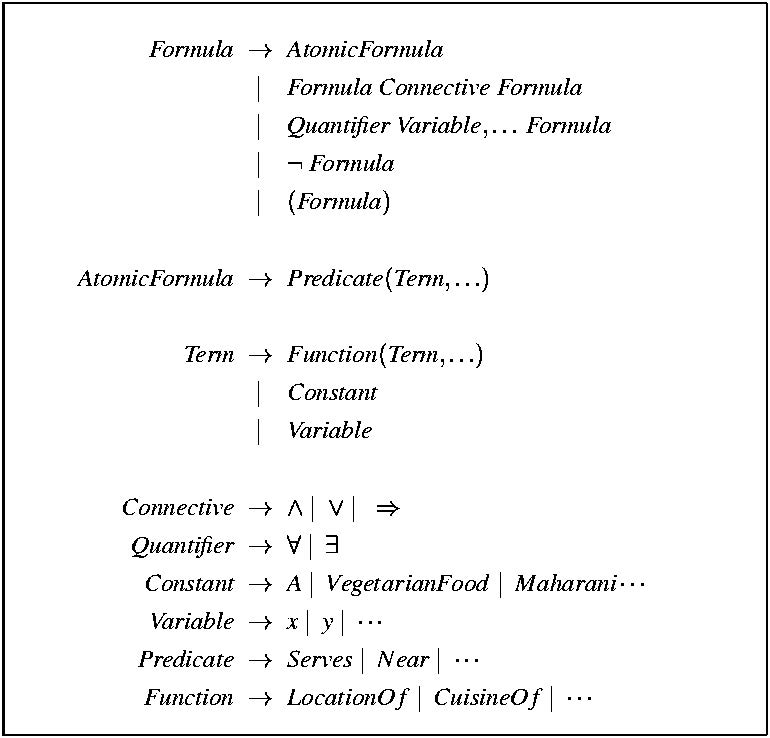
\includegraphics[width=0.7\textwidth]{fol.jpg}
\end{figure}
FOL takes a model-theoretic semantics: a FOL formula is true with respect to a model and an interpretation.\\
Model contains a domain of objects and relations among objects.\\
An interpretation is a mapping:
\begin{itemize}
	\item Constant symbol $\to$ object
	\item Predicate symbol $\to$ relation
	\item Function symbol $\to$ function relation
\end{itemize}
\end{definition}
\begin{definition}[Lambda Expression]
\hfill\\\normalfont A lambda expression is $\lambda x: P(x)$, where $P(x)$ is a FOL formula.\\
$\lambda$-reduction is to apply a lambda expression to a term.
\end{definition} 
\begin{definition}[Inference]
\hfill\\\normalfont We perform inference by modus ponens: $\alpha \land \alpha \implies \beta$ so $\beta$.\\
We call $\alpha$ the antecedent of $\alpha\implies \beta$ and $\beta$ the consequent.
\end{definition}
\begin{definition}[Categories]
\hfill\\\normalfont We use \textbf{reification}, i.e., we represent all concepts that we want to make statements about as full-fledged objects.
\end{definition}
\begin{definition}[Event]
\hfill\\\normalfont We use reification to elevate events to objects, and arguments of an event will apear as predicates.
\end{definition}
\clearpage
\section{Computational Semantics}
\begin{theorem}[Principle of Compositionality]
\hfill\\\normalfont The meaning of a sentence can be composed from the meaning of its parts.
\end{theorem}
The meaning of a setntence is dependent on the ordering, grouping and relations among the words in the sentence(syntactic structure).\\
We will pass inputs throw syntactic analysis and then semantic analysis to get meaning representations as output.
\begin{definition}[Syntax-driven Semantic Analysis]
\hfill\\\normalfont Syntax-driven semantic analysis allows for multiple syntactic parses and multiple meaning representations. It leaves to discourse processing to select among these multiple meaning representations, by using knowledge of context and other domain-specific knowledge.
\end{definition}
\begin{definition}[Semantic Attachments]
\hfill\\\normalfont We augment CFG rules with semantic attachments:
\[
A\to\alpha_1\ldots\alpha_n\;\;\;\{f(\alpha_j\cdot \text{sem}, \ldots, \alpha_k\cdot\text{sem})\}
\]
A semantic attachment describes how to compute the meaning representation of the LHS constituent(A.sem) using the meaning representations of the RHS constituents($\alpha_i\cdot\text{sem}$).\\
It associates complex, function-like $\lambda$-expressions with lexical items. It copies semantic values from children to parents in non-branching rules.
\end{definition}
However, \textbf{idioms} can violate the assumption of compositionality.
\clearpage
\section{Lexical Semantics}
\begin{definition}[Lexeme]
\hfill\\\normalfont Lexeme is an individual entry in the lexicon, which is a pairing of a particular orthographic form and phonological form with a meaning representation.\\
Lexeme is represented by a lemma.
\end{definition}
\begin{definition}[Lemma]
\hfill\\\normalfont Lemma is the grammatical form used to represent a lexeme, often the base form.
\end{definition}
Lexicon is a finite list of lexemes; sense is the discrete representation of the meaning of a lexeme.\\
Some observations include:
\begin{itemize}
	\item Circularity in the definitions, including direct or indirect self-references
	\item Dictionaries are for human consumption but not for computer use
	\item We need grounding in the real-word
	\item But relations among words are still valuable to be studied
\end{itemize}
Relations among lexemes and senses include
\begin{itemize}
	\item Homonymy: a relation that holds between lexemes with the same form but \textit{unrelated} meanings. \\For example, two meanings of the word \textit{bank}
	\item Polysemy: A single lexeme with multiple \textit{related} meanings. \\For example, meanings of the word \textit{serve}.
	\item Metonymy: Denote a concept by naming some other concept closely related to it
	\item Synonymy: a relation that holds between different lexemes with the same meaning.\\
	Two lexemes are considered \textbf{synonyms} if they can be substituted for one another in \textit{some} sentence without changing the meaning/acceptability of the sentence.
	\item Hyponymy: A subclass relation between two lexemes, with is-a hierarchy.
\end{itemize}
\newpage
\begin{definition}[Thematic Roles]
\hfill\\\normalfont Thematic roles are generalized across events, and characterize arguments of verbs.\\
Thematic roles include:
\begin{figure}[h]
\centering
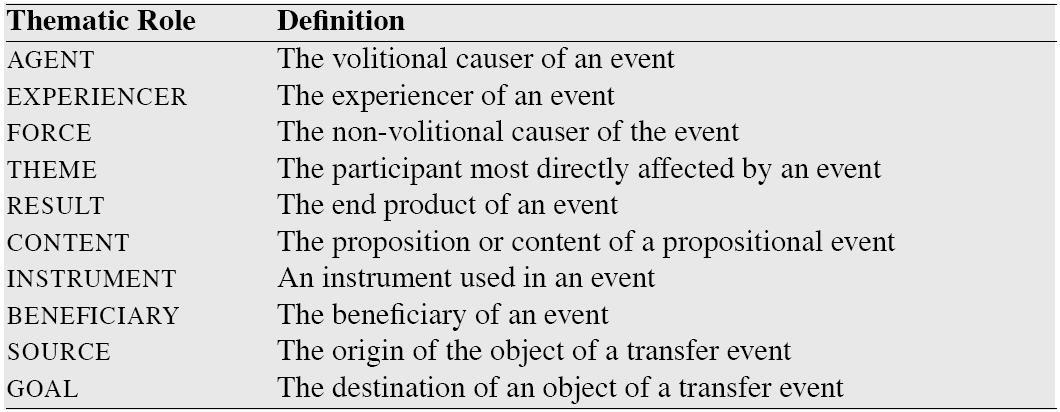
\includegraphics[width=0.7\textwidth]{thematicroles.jpg}
\end{figure}
\end{definition}
Diathesis alternations allows thematic roles to be ambiguous.
\begin{definition}[Metaphor]
\hfill\\\normalfont Metaphor refer to and reason about a concept or domain using words and phrases whose meanings come from a completely \textbf{different} domain.
\end{definition}
\clearpage
\section{Computational Lexical Semantics}
Word Sense disambiguation(WSD) determine the correct sense of a word in context.\\
WordNet is the most widely used online English lexical resources in NLP.\\
We can use Machine Learning to perform robust WSD:
\begin{itemize}
	\item Supervised Learning
	\item Bootstraping
	\item Unsupervised
\end{itemize}
For \textbf{supervised learning} approaches, we take target word, which is the word to be disambiguated and context, in which the target word is embedded, as input.\\
We do preprocessing of context:
\begin{itemize}
	\item POS tagging
	\item Stemming
	\item Parsing
\end{itemize}
and eventually convert into a feature vector representation.\\
We usually extract linguistic features, like collocation features and co-occurrence features.\\
Collocation features are positive specific, and contain local information. Co-occurrence features are words occurring in a fixed size window around the target word, is position-independent and contain global/topical information.\\
Traidtional supervised learning will learn from a manually sense-tagged corpus, using algorithms like Naive Bayes:
\[
\hat{s}=\arg\max_{s\in S}P(s)\prod_{j=1}^n P(v_j\mid s)
\]
Deep Learning uses Bi-LSTM approach: $\text{biLSTM}(x_{1:n}, i)=y_i=[\text{LSTM}^f(x_{1:i}); \text{LSTM}^b(x_{n:i})]$ and $\text{NN}(y_i)=z=g(y_iW^1+b^1)W^2+b^2$, and $o=\text{softmax}(z)$, with categorical cross-entropy loss function. Note that $W^2, b^2$ are specific to each word type.\\
For \textbf{bootstrapping approach}, we have weakly supervised data, and we use Yarowsky algorithm:
\begin{itemize}
	\item Start with supervised training on seed examples
	\item Use trained classifier to label all unlabelled examples
	\item Choose the most confidently labellled examples to add to the growing pool of training examples
	\item Iterate
\end{itemize}
For \textbf{unsupervised methods},
\begin{itemize}
	\item We discover word senses
	\item Group sentences into clusters of similar feature vectors according to some similarity metric
	\item We use agglomerative clustering
\end{itemize}
There are 2 kinds of WSD evaluation:
\begin{itemize}
	\item Extrinsic evaluation:
	\begin{itemize}
		\item In vivo evaluation
		\item Task based evaluation
		\item End-to-end evaluation
	\end{itemize}
	\item Intrinsic evaluation
	\begin{itemize}
		\item In vitro evaluation
	\end{itemize}
\end{itemize}
\clearpage
\section{Computational Discourse}
\begin{definition}[Discourse]
\hfill\\\normalfont Discourse is a coherent structured group of sentences.
\begin{itemize}
	\item Monologue is communication that flows in one direction, from speaker to the hearer
	\item Dialogue allows each participant periodically to take turn to become a speaker/hearer
\end{itemize}
\end{definition}
Note that a randomly ordered sequence of sentences does not form a discourse. Discourse must be \textbf{coherent}.
\begin{theorem}[Rhetorical Structure Theory(RST)]
\hfill\\\normalfont RST is based on 23 rhetorical relations. Most relations hold between two text spans, called a \textit{nucleus} and a \textit{satellite}.\\
Nucleus is the unit that is more central to the writer's purpose, and can be interpretable independently.\\
Satellite is less central and generally only interpretable wrt the nucleus.
\end{theorem}
DIscourse parsing extract a tree/graph representing an entire discourse, with a directed edge from a satellite to its nucleus:
\begin{enumerate}
	\item Identify cue phrases
	\item Segment a text into discourse segments, using cue phrases
	\item Classify the relation betwween each consecutive discourse segment, using cue phrases.
\end{enumerate}
However, problem with above algorithm include:
\begin{itemize}
	\item Cue phrases are ambiguous
	\item Many coherence relations are NOT signaled by cue phrases.
\end{itemize}
\begin{definition}[Reference]
\hfill\\\normalfont Reference is use of linguistic expression to denote an entity.\\
Reference resolution is to determine what entities are referred to by which linguistic expressions.\\
Referring expression is a natural language expression used to perform reference, whereas referrent is the entity referred to.\\
Two referring expressions \textit{corefer} when they are used to refer to the same entity. The first of two is the \textit{antecedent} and the second \textit{anaphor}.\\
\textbf{Anaphora} is reference to an entity that has been previously introduced into the discourse. 
\end{definition}
There are 2 reference resolution tasks:
\begin{itemize}
	\item Coreference resolution: finding referring expressions that refer to the same entity
	\item Pronominal anaphora resolution: finding the antecedent for a single pronoun
\end{itemize}
Coreference chain is the set of coreferring expressions.\\
Types of referring expresisons can be
\begin{itemize}
	\item Indefinite noun phrases, which introduce entities new to the hearer
	\item Definite noun phrases, which refer to entities identifiable to the hearer.
	\item Pronouns, which require referents to have a high degree of salience; usually refer to entities introduced no further than one or two sentences back.\\
	There are 2 types of pronouns
	\begin{itemize}
		\item Cataphora, which are pronouns mentioned before there referrent
		\item Pronouns in quantified contexts, which behaves like a variable bound to a quantified expression
	\end{itemize}
	\item Demonstratives: this, that, these those
	\item Names: names of people/organizations/locations
	\item Inferrables: a referring expression does not refer to any entity that has been explicitly mentioned but instead one that can be inferentially related to a mentioned entity
	\item Generics: a generic reference that does not refer back to an entity explicitly mentioned in the text
	\item Non-referential uses
\end{itemize}
For pronominal anaphora resolution, we check
\begin{itemize}
	\item Number agreement
	\item Person agreement
	\item Gender agreement
	\item Binding theory constraints
	\item Selectional restrictions
	\item Recency
	\item Grammatical role: a salience hierarchy ordered by grammatical position
	\item Repeated mention: entities that have been focused on in the prior discourse are more likely to continue to be focused on in subsequent discourse.
	\item Parallelism
	\item Verb semantics
\end{itemize}
Task for pronominal anaphora resolution is, given a pronoun and potential antecedent NP, determine if pronoun refers to the NP. Training data is hand-labelled corpus in which each pronoun has been linked by hand to its antecedent.\\
Features are those criteria above. We can use LSTM.
Let $g_i$ to be span representation for span $i$, and input sentence with word embeddings to be $x_{1:T}$. Let output vector at position $t$ to be $\text{biLSTM}(x_{1:T}, t)=x_t^\ast = [\text{LSTM}^f(x_{1:t}), \text{LSTM}^b(x_{T:t})]$. We use attentino mechanism to represent head word of the span:\\
let $\alpha_t=w_\alpha\cdot MLP(x_t^\ast)$, $a_{i,t}=\frac{\exp(\alpha_t)}{\sum_{k=\text{START}(i)}^{\text{END}(i)}\exp(\alpha_k)}$.\\
Let $\hat{x}_i=\sum_{t=\text{START}(i)}^{\text{END}(i)}a_{i,t}\cdot x_t$.
Let $\phi(i)$ encode the length of span $i$, then $g_i = [x_{\text{START}(i)}^\ast, x_{\text{END(i)}}^\ast, \hat{x}_i, \phi(i)]$.
Pairwise score $s(i,j)$ for a coreference link between span $i$ and $j$.
\begin{itemize}
	\item $s_m(i)=w_m\cdot MLP(g_i)$
	\item $s_a(i,j)=w_a\cdot MLP([g_i; g_j; g_j\circ g_j; \psi(i,j)])$
	\item $\psi(i,j)$ encodes the distance between two spans
	\item $s(i,j)=\begin{cases}0 &\text{ if }j=\epsilon\\s_m(i) + s_m(j)+s_a(i,j)&\text{ if }j\neq \epsilon\end{cases}$
\end{itemize}
Suppose we have $N$ spans,
\[
P(y_1,\ldots, y_N)=\prod_{i=1}^N P(y_i)=\prod_{i=1}^N \frac{\exp(s(i,y_i))}{\sum_{y'\in y(i)}\exp(s(i, y'))}
\]
where $y_i$ is antecedent for span $i$, and $y(i)$ is set of possible assignments for $y_i$. 
\end{document}